\documentclass{beamer}

\usepackage[utf8]{inputenc}
\usepackage{listings}
\usepackage{tikz}
\usetikzlibrary{fit,positioning}
% \usepackage[style=alphabetic,giveninits=true,terseinits=true]{biblatex}

\definecolor{tumblue}{RGB}{0,101,189}
\definecolor{dkgreen}{rgb}{0,0.6,0}
\definecolor{mauve}{rgb}{0.58,0,0.82}
\lstset{
  basicstyle=\footnotesize\ttfamily,
  columns=fullflexible,
  keywordstyle=\bfseries\color{blue},
  commentstyle=\color{dkgreen},
  stringstyle=\color{mauve},
}

\lstset{frame=tb,
  % language=Rust,
  aboveskip=3mm,
  belowskip=3mm,
  % showstringspaces=false,
  columns=flexible,
  basicstyle={\small\ttfamily},
  numbers=left,
  numbersep=5pt,
  xleftmargin=\parindent,
  numberstyle=\color{gray},
  % keywordstyle=\color{blue},
  % commentstyle=\color{dkgreen},
  % stringstyle=\color{mauve},
  breaklines=true,
  % breakatwhitespace=true,
  tabsize=2
}
\definecolor{cgreen}{RGB}{60,201,65}

% \DeclareFieldFormat{url}{\href{#1}{\resizebox{!}{2ex}{\lower3pt\hbox{\pgfuseimage{beamericononline}}}}}
% \addbibresource{slides.bib}

\setbeamerfont{footnote}{size=\tiny}
\renewcommand\footnoterule{}
\usecolortheme{orchid}
\setbeamertemplate{navigation symbols}{}
\setbeamertemplate{sidebar right}{% also implies no navbar
  \llap{\tikz\fill[tumblue,scale=.1] (0,0) ++(-5cm,-5cm) ++(-10cm,0)
      +(0cm,0cm) -- +(4cm,0cm) -- +(4cm,-4cm) -- +(5cm,-4cm) -- +(5cm,0cm) --
      +(10cm,0cm) -- +(10cm,-5cm) -- +(9cm,-5cm) -- +(9cm,-1cm) --
      +(8cm,-1cm) -- +(8cm,-5cm) -- +(7cm,-5cm) -- +(7cm,-1cm) --
      +(6cm,-1cm) -- +(6cm,-5cm) -- +(3cm,-5cm) -- +(3cm,-1cm) --
      +(2cm,-1cm) -- +(2cm,-5cm) -- +(1cm,-5cm) -- +(1cm,-1cm) --
      +(0cm,-1cm) -- cycle;}
  % Slide number in triangle.
  \vfill\llap{\tikz\path[fill=tumblue,inner sep=3pt] (0,0) -- ++(-1cm,0) -- +(1cm,1cm) -- cycle node[anchor=south east] {\usebeamerfont{footline}\color{white}\bfseries\insertframenumber};}%
  % Variant without triangle
  % \vfill\llap{\usebeamerfont{footline}\usebeamercolor[fg]{footline}\insertframenumber\hskip3pt}\vskip3pt%
}

\title{Ownership types in theory and practice (in Rust)}
\author{Fritz Rehde}
\institute{School of Computation, Information, and Technology\\Technical University of Munich}
\date{26.01.2023}

% \useoutertheme[subsection=false]{miniframes}

\begin{document}

\frame{\titlepage}

\begin{frame}{Overview}
\tableofcontents
\end{frame}

\section{Motivation}

\begin{frame}[fragile]{Memory safety}

C++
\begin{lstlisting}
std::vector<int> v { 10, 11 };
int *vptr = &v[1]; // points into v
v.push_back(12);
std::cout << *vptr; // bug (use-after-free)
\end{lstlisting}

Rust
\begin{lstlisting}
let mut v = vec![10, 11];
let vptr = &mut v[1]; // points *into* v
v.push(12);
println!("{}", *vptr); // compiler error
\end{lstlisting}

\end{frame}

\section{Background}

\subsection{Ownership types in theory}

\begin{frame}{Domain specific terms}
\end{frame}

\begin{frame}{Owners-as-dominators}

\begin{figure}[fragile]
  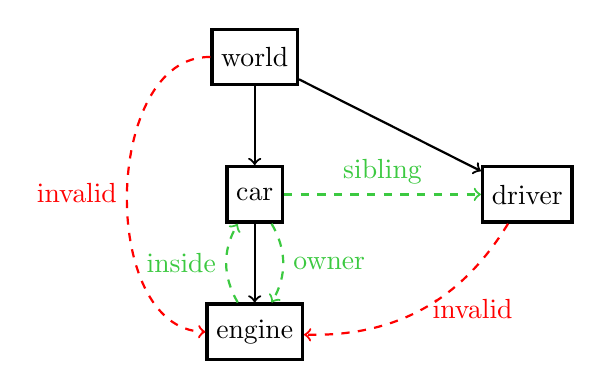
\begin{tikzpicture}[object/.style={rectangle, draw, very thick, minimum size=20}]
    \node[object] (World) {world};
    \node[object] (Car) [below=of World] {car};
    \node[object] (Driver) [right=of Car,xshift=1.5cm] {driver};
    \node[object] (Engine) [below=of Car] {engine};

    \draw[->,thick] (World) to (Car);
    \draw[->,thick] (World) to (Driver);
    \draw[->,thick] (Car) to (Engine);

    \draw[->,thick,dashed,cgreen] (Car) edge[bend left] node[right] {owner} (Engine);
    \draw[->,thick,dashed,cgreen] (Engine) edge[bend left] node[left] {inside} (Car);
    \draw[->,thick,dashed,cgreen] (Car) edge node[above] {sibling} (Driver);
    \draw[->,thick,dashed,red] (World) edge[bend right=90] node[left] {invalid} (Engine);
    \draw[->,thick,dashed,red] (Driver) edge[bend left] node[right] {invalid} (Engine);
  \end{tikzpicture}

  \caption{Owners-as-dominators: Solid lines indicate "owns" and dotted lines indicate "references".}
\end{figure}

\end{frame}

\begin{frame}{Owners-as-modifiers}

\begin{figure}
  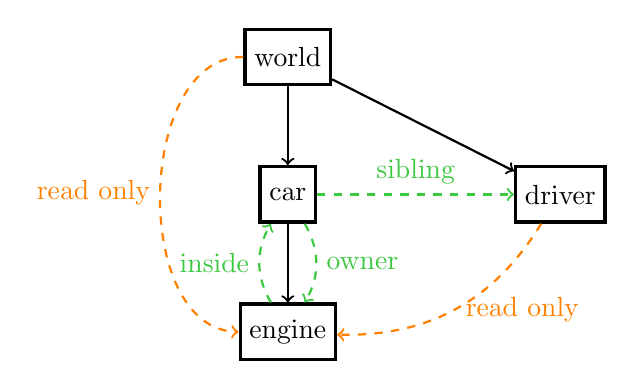
\begin{tikzpicture}[object/.style={rectangle, draw, very thick, minimum size=20}]
    \node[object] (World) {world};
    \node[object] (Car) [below=of World] {car};
    \node[object] (Driver) [right=of Car,xshift=1.5cm] {driver};
    \node[object] (Engine) [below=of Car] {engine};

    \draw[->,thick] (World) to (Car);
    \draw[->,thick] (World) to (Driver);
    \draw[->,thick] (Car) to (Engine);

    \draw[->,thick,dashed,cgreen] (Car) edge[bend left] node[right] {owner} (Engine);
    \draw[->,thick,dashed,cgreen] (Engine) edge[bend left] node[left] {inside} (Car);
    \draw[->,thick,dashed,cgreen] (Car) edge node[above] {sibling} (Driver);
    \draw[->,thick,dashed,orange] (World) edge[bend right=90] node[left] {read only} (Engine);
    \draw[->,thick,dashed,orange] (Driver) edge[bend left] node[right] {read only} (Engine);
  \end{tikzpicture}

  \caption{Owners-as-modifiers: Solid lines indicate "owns" and dotted lines indicate "references".}
\end{figure}

\end{frame}


\section{Concept}

\subsection{Ownership in Rust}

\begin{frame}{Memory allocation system}

\end{frame}

\begin{frame}{Transferring ownership}
\end{frame}

\begin{frame}{References and borrowing}
\end{frame}

\section{Evaluation}

\subsection{Another ownership implementation}


\section{Conclusions and outlook}

\begin{frame}
  Here are some conclusions.
\end{frame}


\end{document}
